\documentclass{article}

\usepackage{arxiv}

\usepackage[utf8]{inputenc} % allow utf-8 input
\usepackage[T1]{fontenc}    % use 8-bit T1 fonts
\usepackage{hyperref}       % hyperlinks
\usepackage{url}            % simple URL typesetting
\usepackage{booktabs}       % professional-quality tables
\usepackage{amsfonts}       % blackboard math symbols
\usepackage{nicefrac}       % compact symbols for 1/2, etc.
\usepackage{microtype}      % microtypography
\usepackage{lipsum}		% Can be removed after putting your text content
\usepackage{amssymb,amsmath}
\usepackage{listings}
\usepackage{graphicx}
\usepackage{subfig}
\usepackage{apacite}

\title{Contact-tracing strategies for SARS-CoV-2 eradication
\textbf{**** UNFINISHED DRAFT ****}
}

%\date{September 9, 1985}	% Here you can change the date presented in the paper title
%\date{} 					% Or removing it

\author{
  Daniel Tang\\
  Leeds Institute for Data Analytics\thanks{This project has received funding from the European Research Council (ERC) under the European Union’s Horizon 2020 research and innovation programme (grant agreement No. 757455)}\\
  University of Leeds\\
  Leeds, UK\\
  \texttt{D.Tang@leeds.ac.uk} \\
  %% examples of more authors
  %% \AND
  %% Coauthor \\
  %% Affiliation \\
  %% Address \\
}


\begin{document}
\maketitle

\begin{abstract}
As of $27^{th}$ March a large and increasing proportion of the global population are living under social distancing measures in order to control the spread of COVID-19. If these measures are successful we will, in a few months, be in a situation where prevalence is again low in certain parts of the world, however, it is not clear what the best policy will be at that point. This paper investigates the feasibility of using contact tracing along with a combination of other measures in order to ease the social distancing measures while preventing a resurgence of the disease.

\textbf{**** THIS IS UNFINISHED RESEARCH WHICH MAY CONTAIN ERRORS AND IS SUBJECT TO CHANGE ****}
\end{abstract}

% keywords can be removed
\keywords{COVID-19, SARS-CoV-2}

\section{Introduction}

Many countries in the world are now committed to a surge in incidence of COVID-19 and are practising social distancing in order to suppress its spread. If successful, these countries will soon be in a situation where prevalence is reducing. Once this is achieved there are a number of strategies:
\begin{itemize}

\item lift the social distancing measures and allow a second (and subsequent) waves until herd immunity is achieved\cite{ferguson2020impact}.

\item maintain low levels until a vaccine is available

\item eradicate the virus locally and impose strict border controls and containment strategies until the virus is contained globally
\end{itemize}

Here we investigate the feasibility of the third option by slowly lifting social distancing measures while maintaining self isolation of symptomatic individuals and implementing an extensive testing and contact-tracing capability.

\section{Description of the Model}

The model we use is an agent-based discrete event simulation. It is based on the stochastic branching model described in \cite{hellewellfeasibility} but modified in order to capture enough detail to explore different testing and contact-tracing strategies\footnote{Although a discrete-event simulation is slower than a branching model, execution time is not a bottleneck so it is worthwhile in order to capture the dynamics.}.

The model consists of infected agents, each of which belongs to a household and a workplace/school. Once infected, an agent goes though an incubation period with duration drawn from a Weibull distribution (with shape parameter $2.322737$ and scale parameter $6.492272$)\cite{backer2020incubation}. The transmission serial interval (i.e. time from exposure to transmission) is drawn from a skew normal distribution with location parameter equal to the clinical onset time (i.e. end of the incubation period), scale parameter of 2.0 and skew parameter of 1.95\cite{hellewellfeasibility}. This results in 15\% of infections occurring before clinical onset\cite{hellewellfeasibility}. In order to avoid unrealistically early transmissions, the serial interval was bounded to a minimum of 1 day. At creation, $17.9\%$ of agents are deemed to be asymptomatic\cite{:/content/10.2807/1560-7917.ES.2020.25.10.2000180}\footnote{[TODO: Age weight this figure]}. Asymptomatic carriers are assumed to be $\frac{2}{3}$ as infectious as symptomatic carriers\cite{ferguson2020impact}. The number of susceptible agents that an infected agent will infect if not isolated is drawn from a negative binomial distribution with overdispersion parameter $10.0$\cite{zhuang2020preliminary}\cite{riou2020pattern} and mean of $\frac{3R_0}{3 - \rho}$ for symptomatic agents and $\frac{2R_0}{3 - \rho}$ for asymptomatic agents where $\rho=0.179$ is the probability of being asymptomatic and $R_0$ is the basic reproductive number. If an agent is isolated, any transmission events that occur after isolation will not result in the creation of another infected agent.

Each transmission event occurs either in the household, at the workplace/school or in the community. This allows us to capture the differences in ease and speed of contact tracing in these three cases, and to capture the effect of different policies for tracing in these contexts. It also allows us to capture the effect of household-wide self-isolation policies such as those implemented in the UK. The relative probability of transmission in the three locations was calibrated in order to obtain equal aggregate numbers of transmission events in each location, following \cite{ferguson2020impact}. The distribution of number of members in a household was calibrated against\cite{smithHouseholds}.

In order to account for people who have already been infected during the first wave of infection, a proportion of the population is immune to infection. A transmission event to an immune agent does not cause infection. This immunity is applied only to school/workplace and community under the assumption that, during the peak, under ``stay at home'' rules, if one member of a household contracts the disease it is highly likely that all other members will also contract it, and so the whole household will become immune. This means that only members of non-immune households can subsequently become infected.

\subsection{Contact tracing and isolation policy}

It was assumed that a ``self-isolate'' policy was in place such that anyone who becomes symptomatic must self-isolate and report to authorities. At this point all members of that person's household must also self-isolate. It was assumed that there was a delay between symptom onset and self-isolation/reporting. Once reported, all members of the household are tested and those that test positive are contact-traced. Contact tracing was assumed to identify $90\%$ of contacts in the workplace/school and $10\%$ of contacts in the community. Symptomatic contacts in the workplace must isolate immediately, other contacts are tested and must isolate on positive test result. The time for a test result to be processed was assumed to be 24 hours. It was assumed that $10\%$ of the population do not comply with these rules and never self-isolate or report themselves.

The source code of the model is available at \href{https://github.com/danftang/Covid19}{https://github.com/danftang/Covid19}

\section{Preliminary results}

Simulations were carried out to find the probability that an initial population of 100 infected agents could be eradicated under different scenarios. Eradication was deemed to have been achieved if the cumulative number of cases remained below 5000 and there was no untraced infected population at 15 weeks into the simulation. $R0$ was set to $2.4$\cite{ferguson2020impact} and it was assumed that $5\%$ of the population was immune. The probability of eradication was estimated by performing a monte-carlo run of 300 simulations and counting the proportion that achieved eradication.

It was found that the probability of eradication was highly sensitive to the delay between symptom onset and self-isolation, and to the time after exposure that an infected person would test positive, so monte-carlo runs were performed for a range of values of these parameters. Figure \ref{onsetToIsolation} shows the probability of eradication against the delay between symptom onset and self-isolation while figure \ref{exposureToPositiveTest} shows the probability of eradication against the delay between exposure and positive test result.

\begin{figure}
\begin{center}
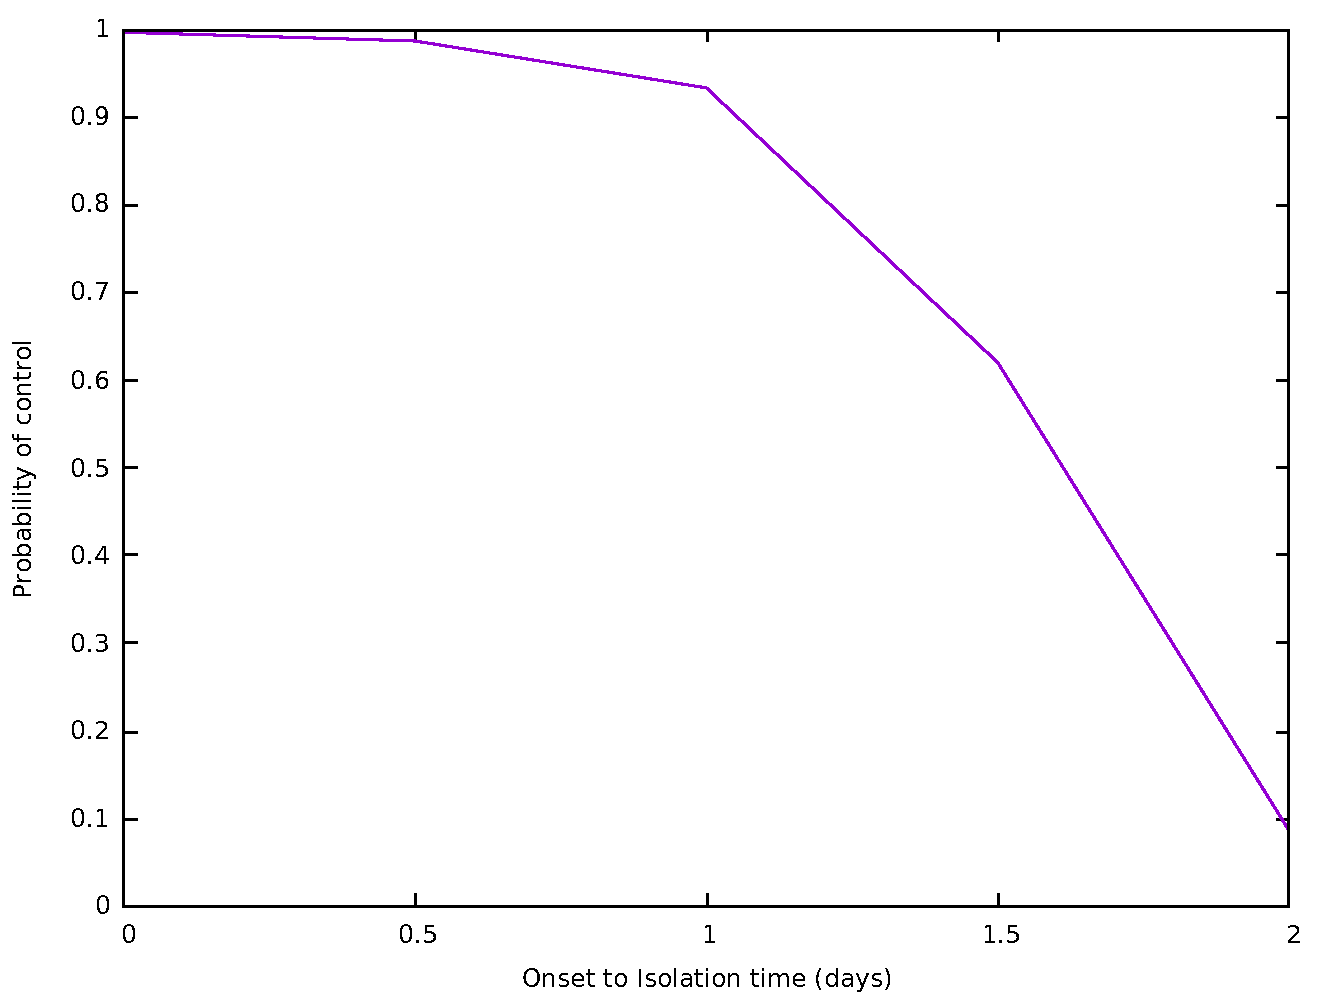
\includegraphics[width = 10cm]{onsetToIsolation.pdf}
\end{center}
\caption{Probability of eradication for different delays between the onset of symptoms and self-isolation, assuming all infected test positive.}
\label{onsetToIsolation}
\end{figure}

\begin{figure}
\begin{center}
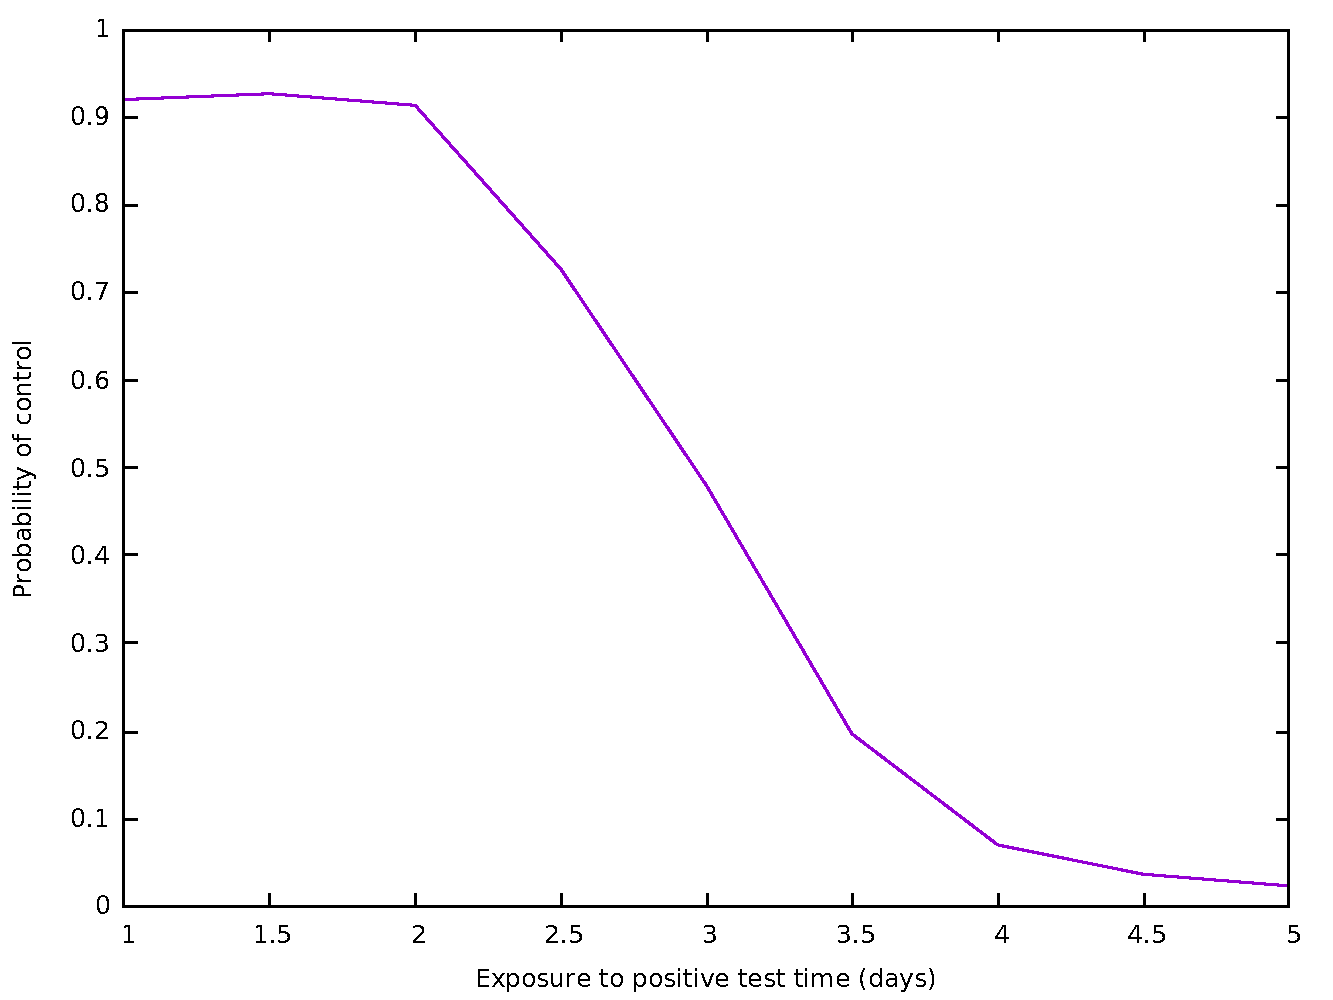
\includegraphics[width = 10cm]{exposureToPositiveTest.pdf}
\end{center}
\caption{Probability of eradication for different delays between exposure and a test result becoming positive, assuming a delay of 1 day between symptom onset and self-isolation.}
\label{exposureToPositiveTest}
\end{figure}

\section{Discussion}

These early results are subject to further calibration of the model and are likely to change as our understanding of the dynamics of SARS-CoV-2 develops. It also remains to do a proper sensitivity analysis of the model, and to properly treat uncertainty, which is large. However, they do indicate that while it is not impossible in theory for contact-tracing to be effective, a very high proportion of the population will have to isolate, or be isolated, within 1 day of symptom onset. This will be difficult to achieve in practice, and so for contact tracing to work, it is likely that it will have to be implemented in combination with some other policy or policies to suppress community transmission. Our ongoing research will investigate these possibilities.

\pagebreak
%\bibliographystyle{unsrtnat}
%\bibliographystyle{apalike} 
\bibliographystyle{apacite}
\bibliography{references}

\end{document}
